% Requires:
% \providecommand{\glsxtrshort}[1]{#1}
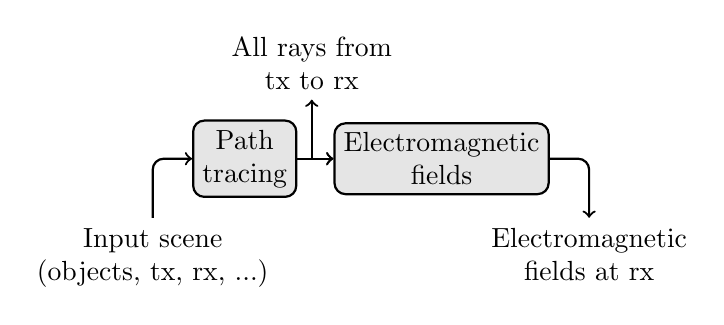
\begin{tikzpicture}  % Should fit in one column
  \tikzset{block/.style={draw=black, thick, align=center, rounded corners, minimum height=0.5cm, fill=gray!20, text=black}}
  \node[block] (rt) at (0,0) {Path\\tracing};
  \node[block] (em) at (2.5,0) {Electromagnetic\\fields};
  \draw[<-,thick, rounded corners] (rt.west) -| ++(-.5, -.75) node[below, align=center] {Input scene\\(objects, \glsxtrshort{tx}, \glsxtrshort{rx}, ...)};
  \draw[->, thick] (rt.east) -- (em.west);
  \draw[->, thick] (rt.east) -- (em.west) coordinate[pos=.4] (midway) {};
  \draw[->, thick] (midway) -- ++(0, +.75) node[above, align=center] {All rays from\\\glsxtrshort{tx} to \glsxtrshort{rx}};
  \draw[->, thick, rounded corners] (em.east) -- ++(+.5, 0) -- ++(0, -.75) node[below, align=center] {Electromagnetic\\fields at \glsxtrshort{rx}};
\end{tikzpicture}
